\section*{Modeling sequential variable}

The basic idea is to cast the model in terms of conditional transition probabilities $Pr(y_{i} = j | y_{i} >= j), j=1, \ldots, J-1$. In our application, this is the characteristic of the $i^{th}$ woman who has first birth in interval $j$, which occurs only after passing levels 1, 2, $\ldots$, $j-1$ and only bears at level $j$ or higher. The probability of having birth at interval $j$, conditional on the event that the $j$th interval is reached is given by:

\begin{align}
	Pr(y_{i} = j | y_{i} >= j, w_{i})= F(\theta_{j} - w_{i};'\alpha), j=1, \ldots, J-1,
\end{align}}

where $\theta = (\theta_{1}, \ldots, \theta_{J-1})$ are the cutpoints, one of which is normalized to 0 to ensure identifiability. $F$ is a strictly monotone function, $w_{i}'\alpha$ is the effect of covariates associated with the response. If $F$ is chosen to be a logistic distribution function we obtain a sequential logit (Tutz 2003; Liu and Agresti 2005),

\begin{align}
	Pr(y_{i}=j | y_{i} >= j, w_{i}) = \frac{exp(\theta_{j} - w_{i}'\alpha)}{1+exp(\theta_{j} - w_{i}'\alpha)},
\end{align}

or equivalently in logit form

\begin{align}
	n_{ij} = log \frac{Pr(y_{i} = j |w_{i})}{Pr(y_{i}>j | w_{i})} = \theta_{j} - w_{i}'\alpha, j=1, \ldots, J-1
\end{align}

where $n_{ij}$ is a predictor.

The above model can also be formulated in terms of latent variables expressing the propoensity of a women to reach category $j$ before bearing her first child. Corresponding to the $j$th category (of time to first birth), definte latent variable \{$z_ij$\}, where $z_{ij} = \theta_{j} - w_{i}'\alpha + \epsilon_{ij} = n_{ij} + \epsilon_{ij}$, where $\epsilon_{ij}$ is an error variable.

We observe $y_{i} = 1$ if $z_{i1} <= \theta_{1}$, and we observe $y_{i}=2$ if the first latent variable $z_{i1} > \theta_{1}$ and the second latent variable $z_{i2} <= \theta_{2}$. In general we have:

The latent variable representation can be simplified by incorporating cutpoints

To model \emph{State- and Opposition-Focused ICC Transition} we need to account for the sequential way in which states and opposition actors transition through the ICC process (i.e., no ICC investigation, preliminary, and formal). Typically, scholars would use an ordinal regression framework to model such processes. In these models, the probability of interest is the cumulative probability, which is the probability at or below a given outcome category. For example, if income is grouped into four intervals -- 1 = $< \$25,000$; 2 = $\$25,000 to <\$50,000$; 3 = $\$50,000 to <\$75,000$; 4 = $>=\$75,000$ -- the cumulative probability for category 2 is the probability that a respondent is located in one of the two bottom income categories. For an outcome with ($y$) with four categories (1-4), $y$ is linked to the binary outcomes in the cutpoint equations ($y_{1} - y_{3}$) by the measurement equations:

\begin{eqnarray}
	y_{1} =
	\begin{cases}
	1 \text{ if } y = 1 \nonumber \\
	0 \text{ if } y = 2-4 \nonumber \\
\end{cases}
	y_{2} =
	\begin{cases}
	1 \text{ if } y = 1-2 \nonumber \\
	0 \text{ if } y = 3-4 \nonumber \\
\end{cases}
	y_{3} =
	\begin{cases}
	1 \text{ if } y = 1-3 \nonumber \\
	0 \text{ if } y = 4 \nonumber \\
\end{cases}
\end{eqnarray}

The sample size does not change across the cutpoint equations, which is a feature of cumulative models.

The probability of interest in stage models is the conditional probability ($Pr[ y = m | y >= m]$), which is the probability for a particular category, $m$, given the respondent is in that category or a higher one. As a result, respondents in lower categories are excluded. For example, if the dependent variable is a four-category measure of educational attainment -- 1 = less than high school; 2 = high school; 3 = some college; and 4 = college or more -- the conditional probability for category 2 is the probability that a respondent has a high school degree given that he or she has a high school degree or more. We use Fullerton's (2009) terminology in referring to this as the "stage" approach because the cutpoint equations represent a series of stages. In order to reach a particular category, respondents must pass through each of the previous categories.\footnote{Stage models are also referred to as "continuation ratio" models (Feinberg 1980; Long 1997; Agresti 2010; Tutz 2012) because the focus is on the sequential process of continuing from one stage to the next. }

For stage models there must be a logical starting point, respondents must pass through earlier stages to reach a later stage, and the stages must be irreversible (Tutz 1991).

For an outcome ($y$) with four categories (1-4), $y$ is linked to the binary variables in the cutpoint equations ($y_{1} - y_{3}$) by the measurement equations:

\begin{eqnarray}
	y_{1} =
	\begin{cases}
	1 \text{ if } y = 1 \nonumber \\
	0 \text{ if } y = 2-4 \nonumber \\
\end{cases}
	y_{2} =
	\begin{cases}
	1 \text{ if } y = 2 | y >= 2 \nonumber \\
	0 \text{ if } y = 3-4 | y >= 2 \nonumber \\
\end{cases}
	y_{3} =
	\begin{cases}
	1 \text{ if } y = 3 | y >= 3 \nonumber \\
	0 \text{ if } y = 4 | y >= 3 \nonumber \\
\end{cases}
\end{eqnarray}

The outcomes in the first cutpoint euqations ($y_{1}$) is the same in the cumulative and staghe models. However, the remaining cutpoint equations are different. In addition, the sample size becomes progressively smaller in later stages.

The parallel continuation ratio model treats the ordinal outcome as a series of stages with effects that are constrained to remain constant across stages. In other words, the parallel regression assumption is imposed for every variable. One important difference between cumulativel and stage models is that in stage models higher categories of $y$ may only be reached after successfully proceeding through the lower categories. Scholars do not typically use stage models to analyze variables such as self-rated healath because there is no natural starting point, and one does not need to experience poor or fair health before good or excellent health.

The key assumption in all stage models is that the errors are independent across stages or cutpoint equations (Maddala, 1983). For a three-category outcome with two equations, 1 versus 2-3 and 2 versus 3, we must assume that there is no correlation between the errors in the first and second equations. In other words, the smaller sample in the second equation is a random subset of the larger sample in the first equation. Unfortunately, this may not be a realistic assumption for some ordinal outcomes, such as educational attainment. If the subsamples in later stages are systematically different with respect to unobserved or omitted variables, then the coefficients in later stages may be biased. For instance, the finding of weakening family background effects on educational attainment in later stages is due in part to this type of sample selection bias. The group that successfully makes several transitions to the later educational stages is much more homogeneous than the initial group of respondents.

Coefficients may also vary across cutpoint equations in stage models due to heteroscedasticity of the conditional variances of the latent dependent variables (Cameron and Heckman 1998; Mare 2006). Partial models are ordered regression models that relax the parallel regression assumption for one subset of variables. Relaxing the parallel assumption allows the coefficients in this group to vary across the cutpoint equations. In other words, some variables will have coefficients that change depending on the level of the dependent variable.

Using MLE for ordered regression models is not immune to problems. Although McCullagh (1980) and Pratt (1981) show that the log-likelihood function in ordered regression models has global concavity under general conditions, the numerical estimation of these models can occasionally be problematic in practice. When the overall sample size is small, for example, the estimation of ordered regressional models could fail to reach convergence (McCullagh 1980) or to produce parameter estimates with less-than-optimal properties that are largely unknown. Long (1997)

Specifically, both transition variables can only face a formal investigation after a preliminary has begun.

More formally, in order for actor $i$ to receive a value of $j$ for $Y_{i}$, the actor must pass through all levels less than $j$. The probability of then reaching $j$, conditional on the event that the $j^{th}$ level is reached, is given by:

\begin{eqnarray}
	Pr(y_{i}={j} | Y_{i} \geq {j}, \gamma, \beta) &=& F(\gamma_{j} - x_{i}^{'}\beta) \nonumber \\
	Pr(Y_{i}={j}|\gamma_{1},\beta) &=& F(\gamma_{j} - x_{i}^{'}\beta)\text{ }\prod^{j-1}_{k=1}\text{ }\{1-F(\gamma_{k}-x_{i}^{'}\beta)\} \nonumber
\end{eqnarray}

$\gamma = (\gamma_{1},...,\gamma_{J-1})$

\begin{eqnarray}
	Pr(y_{i}=J|\beta_{1},\gamma) &=&\text{}\prod^{J-1}_{k=1}\text{ }\{1-F(\gamma_{k}-x_{i}^{'}\beta)\} \nonumber
\end{eqnarray}

Latent variable representation

\begin{eqnarray}
	w_{ij} &=& x_{i}^{'}\beta+\epsilon_{ij},\text{ }\epsilon_{ij} \sim iid \nonumber
\end{eqnarray}

Observe:

\begin{eqnarray}
	y_{i} = 1\text{ iff } w_{i1} \leq \gamma_{1} \nonumber \\
	\nonumber \\
	y_{i} = 2\text{ iff }
	\begin{cases}
	w_{i1} > \gamma_{1} \nonumber \\
	w_{i2} \leq \gamma_{2} \nonumber \\
\end{cases}
\end{eqnarray}

Likelihood function:

\begin{eqnarray}
	L(\gamma,\beta) = \prod_{i\colon y_{i}<J}\text{ }[ F(\gamma_{y_{i}} - x_{i}^{'}\beta)\text{ }\prod_{k=1}^{y_{i}=1}\text{ }\{1-F(\gamma_{R}-x_{i}^{'}\beta)\}] &\times \displaystyle \prod_{i\colon y_{i}=J}\text{ }[\prod_{k=1}^{J=1} \{1-F(\gamma_{2} - x_{i}^{'}\beta)\}] \nonumber \\
	\nonumber \\
	(\gamma,\beta) \sim \pi (\gamma,\beta) & \nonumber \\
	\beta \sim N(\beta_{0},\Sigma_{0}) & \nonumber \\
	\nonumber \\
	z_{ij} = w_{ij} - \gamma_{j}, & \nonumber
	\end{eqnarray}
	So...
	\begin{eqnarray}
	y_{i} =
	\begin{cases}
	1\text{ if }z_{i} \leq 0 \nonumber \\
	2\text{ if }z_{i1} > 0, z_{i2} \leq 0 \nonumber \\
	\vdots \nonumber \\
	J-1\text{ if }z_{i1} > 0,...,z_{i,j-2}>0,z_{i,j-1}\leq0 \nonumber \\
	J\text{ if }z_{i1}>0,...,z_{i,j-1}>0
\end{cases}
\end{eqnarray}

Sample from the joint posterior of $(\{z_{ij}\},\beta)$ by ??? sampling of ???:

\begin{eqnarray}
	(\{z_{ij}\} | y,\beta)\text{ and }(\beta,|\{z_{ij}\},y) \nonumber \\
	(\{z_{ij}\} | y,\beta)\stackrel{iid}{\sim}TN_{(a,b)}(\beta,1) \nonumber \\
	\nonumber \\
	(\beta | \{z_{ij}\},y)\stackrel{iid}{\sim}N(\hat{\beta},\hat{\Sigma}) \nonumber \\
	\nonumber \\
	\hat{\beta} = (\Sigma_{0}^{-1}+\sum_{i=1}^{n} x_{i}^{'}x_{i})^{-1} \times (\Sigma_{0}^{-1}\beta_{0}+\sum_{i=1}^{n} x_{i}^{'}z_{i}) \nonumber \\
	\hat{\Sigma} = (\Sigma_{0}^{-1} + \sum_{i=1}^{n} x_{i}^{'}x_{i})^{-1} \nonumber
\end{eqnarray}

\section*{Empirical Results}

\begin{figure}
    \centering
    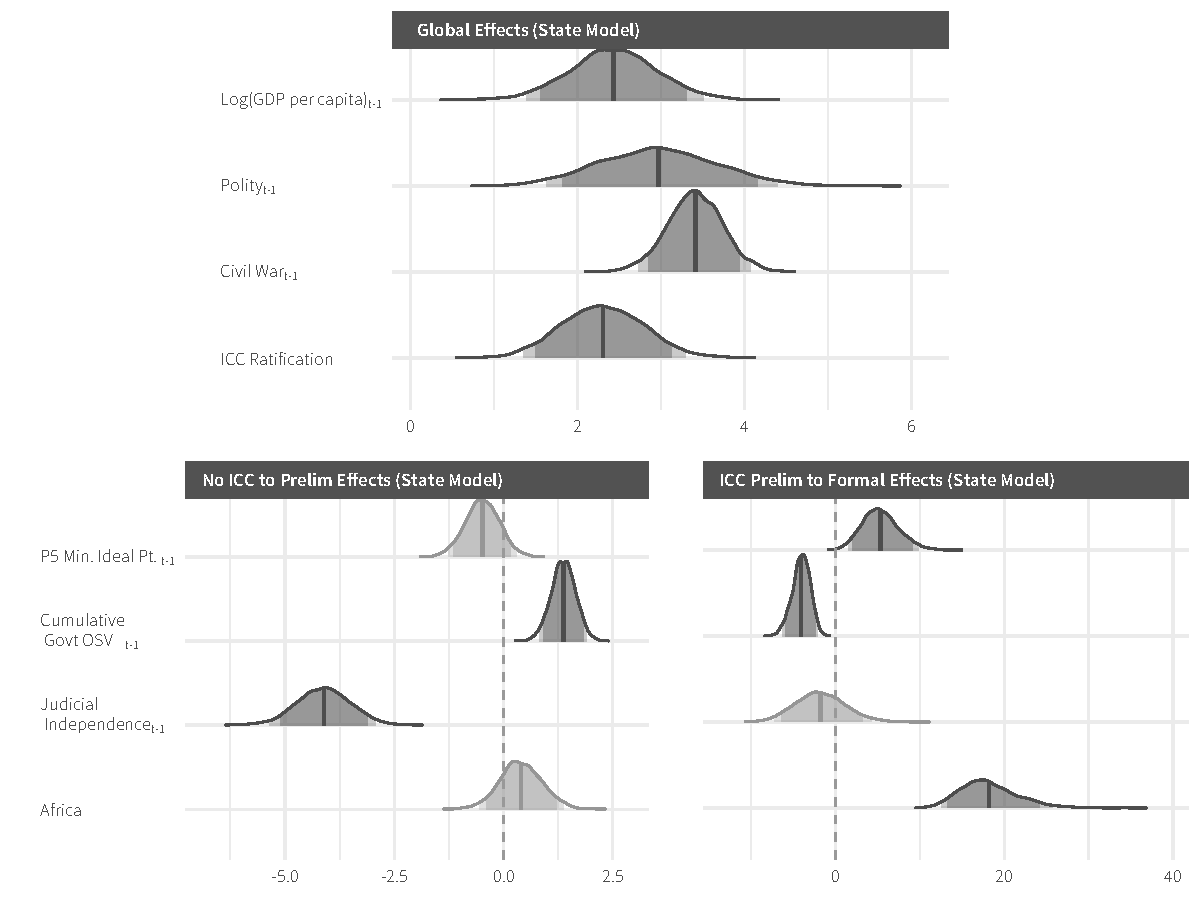
\includegraphics[width=1\textwidth]{stateCoefSumm.pdf}
    \caption{Parameter estimates from State-Focused ICC Transition model visualized through posterior distributions with median values designated by vertical line, lightly shaded portion indicating the 95\% credible interval, and darker shaded portion the 90\% credible interval.}
    \label{fig:stateModel}
\end{figure}

\begin{figure}
    \centering
    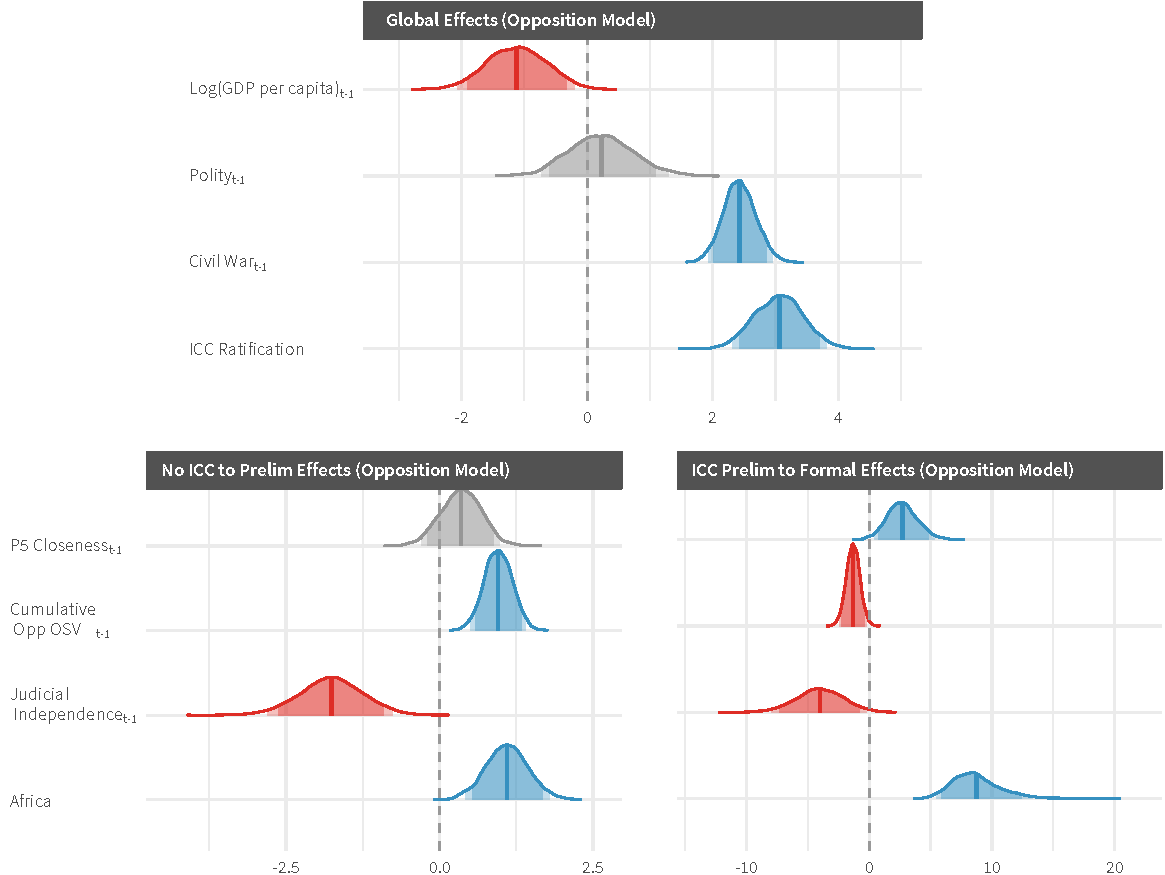
\includegraphics[width=1\textwidth]{rebelCoefSumm.pdf}
    \caption{Parameter estimates from Opposition-Focused ICC Transition model visualized through posterior distributions with median values designated by vertical line, lightly shaded portion indicating the 95\% credible interval, and darker shaded portion the 90\% credible interval.}
    \label{fig:rebelModel}
\end{figure}

% what variables are mostly impactful
% everything from africa down

\subsection*{Onset Models}

In Figure 1, we present the results for the state and rebel focused ICC escalation models.

We first discuss the results for the onset of ICC involvement directed against governments.  Perhaps most significantly, we find no statistical support for the impact of Africa on the onset of such examinations. This result is important given conventional wisdom, which suggests that the ICC and OTP are biased against African states and groups.  The underlying data support this finding; the ICC has initiated 19 investigations against governments or governments and subnational actors, but only 5 involve African states. Thus, both the statistical results and basic trends in the data do not indicate that the ICC has an African bias, at least in this initial stage of ICC involvement.

We find mixed support for the legal mandate variables.  As expected, we see that the government OSV variable is positive and statistically significant. In line with our argument on the ICC’s mandate, this suggests that the OTP is more likely to start a preliminary examination against governments that have intentionally killed more civilians since 2002.  In contrast, we fail to find support for the rule of law variable. This results is largely as expected; as discussed in the theory section above, a strong, independent judiciary may only prevent the escalation of ICC involvement to the formal investigation stage. We discuss this result in greater detail below, where tests allow us to more directly examine the effect of an independent judiciary on the specific decision to initiate a formal investigation. Thus, the results provide some support for the legal mandate argument.

We find little support for the measures that proxy the institutional constraints logic, including the P5 intervention variables, P5 alliance variable, and P5 affinity measure. The results appear to suggest that the OTP’s decision to start a preliminary examination is not based on factors associated with P5 interests.  Nonetheless, it is important to interpret the results with some caution for at least two reasons. First, the small number of cases (i.e. 19 preliminary examinations) makes it difficult to find statistical significance for the key variables. Second, we are unable to include any economic factors, such as trade and foreign aid due to data limitations. There is no data on economic factors that goes to 2015, the last year in our data set. We therefore cannot make any strong claims about the relationship between P5 economic interests and the probability of preliminary examinations.\footnote{In preliminary analyses, we find that higher levels of foreign aid are associated with a lower probability of ICC preliminary examinations.  We plan to pursue this finding in greater detail in the next iteration of the paper.}

Finally we observe mixed results for the control variables. The civil war variable is positive and significant, suggesting that the OTP is more likely to start preliminary examinations in the context of civil wars. We also see that the democracy variable is positive which indicates that the OTP is more likely to initiate preliminary examinations against democratic governments compared to nondemocratic ones.  The ICC ratification variable is positive as expected but it fails to reach standard levels of significance.

We also see mixed results in the model predicting opposition-focused ICC onset. While the Africa variable is positive as expected, it fails to reach standard levels of significance. The underlying data once again reinforces the statistical finding. Among the 15 cases of opposition-based preliminary examinations, only 7 of them involve groups from African states. Consistent with the results from the government model, this finding challenges the conventional wisdom that the ICC has an African bias when it comes to initiating preliminary examinations.

We see strong results for the legal mandate variables. The opposition one-sided violence variable is positive and statistically significant which suggests that the OTP is more likely to start preliminary examinations against opposition groups when they kill more civilians. We also see that the rule of law measure is negative and statistically significant. Consistent with our expectations, this indicates that the OTP is unlikely to start preliminary examinations against opposition groups when the state in question has a strong, independent legal system.

We, however, see little consistent support for the strategic variables. The P5 intervention variables, P5 affinity scores, and P5 alliance variables all fail to reach significance in this model. Consistent with the government models, this suggests that P5 interests fail to explain the OTP’s decision-making in the preliminary examination stage.  As suggested above, however, it is important to interpret these results with some caution given the small number of cases.  Finally, we again observe mixed support for the control variables. The democracy variable is positive and significant, while the other controls fail to reach standard levels of significance.

\subsection*{Escalation Model}

In Table 2, we present the results for the escalation models. We first discuss the findings for the government model.  Overall, we find very strong and consistent results in this model.  First, consistent with prevailing thought, the Africa variable is positive and significant, which suggests that the ICC is more likely to escalate its involvement against African states than governments from other states.

In addition, we see strong support for the legal mandate variables, as both the rule of law and government one-sided violence variables are statistically significant and in the expected direction. The result for the rule of law variable is important, because it suggests that complementarity is an important predictor of greater ICC involvement. As expected, the Court appears to be using the preliminary examination stage to determine if it has jurisdiction in a situation, including whether the state in question has the willingness and capability to investigate perpetrators on its own.

In contrast to the preliminary examination stage, we observe strong results for the realist variables here.  The pro-government interventions variable is negative as expected, while the pro-opposition interventions measure is positive.  Consistent with our argument, the P5 UNGA affinity variable is positive, and P5 alliance ties variable is negative. All four variables clearly indicate that P5 ties influence the ICC decision-making.  Simply, the ICC appears to be less likely to escalate its involvement when the government in question has strong ties with P5 actors.  In other words P5 interests appear to deter greater ICC involvement in situations under preliminary examination.

The control variables also produce significant results; civil war is negative and significant, while both democracy and ICC ratification are positive and significant. The result for ongoing civil war may reflect the fact that the ICC is less capable of carrying out an effective investigation in a country that has ongoing conflict.  Conflict makes it difficult for investigators to safely enter the country and collect information, therefore making it difficult for the OTP to build a strong enough case to progress to issuing indictments, holding hearings, etc.

The opposition model also produces strong findings in this stage (Table 2). As expected, the Africa variable is positive and significant, suggesting that the ICC is more likely to escalate its involvement against opposition groups who reside in Africa. While this finding is largely consistent with the African bias, it is important to interpret it in combination with the results from the onset stage, which suggest that there is not an Africa bias in the preliminary examination stage.  Nonetheless, we see evidence of an Africa bias in this stage.

We also observe strong results for the legal mandate variable in the opposition model. Consistent with the onset stage, both one-sided violence and the rule of law variables are significant and in the expected direction.  This provides strong evidence to suggest that the Court abides by the principle of complementarity and its mandate to prosecute the gravest offenders of human rights violations, such as civilian victimization.

We see mixed results for the realist variables here. In contrast to our expectations, the pro-opposition intervention variable is positive and significant. The surprising result for this variable requires additional research to further clarify the relationship between these types of interventions and ICC involvement against opposition groups.  As expected, we see that both the pro-government interventions and the P5 alliance variables are positive and statistically significant. This suggests that P5 links once again influence the behavior of the ICC. Here, however, we see that strong ties between governments and the P5 can motivate the ICC to escalate its investigations against opposition groups.

We again find mixed support for the control variables; democracy is negative and statistically significant, while ICC ratification is positive and significant as expected. In contrast, we see no support for the civil war variable.

\subsection*{Post-estimation Substantive Results}

The statistical results provide strong support for our legal mandate argument. We also find support for the Africa and realist variables in the escalation model. In this section, we present the post-estimation results for the statistically significant variables in the escalation equation.  We report the results in Table 4. As a reminder, the response variable in this model is a six category variables that measures different levels of ICC involvement in situations. We thus use ordered probit to estimate this model. This estimator produces separate predicted probabilities for the different categories of the response variable.  For the sake of parsimony, we only present the predicted probabilities for the onset of formal investigation category. This is because the predicted probabilities are largely consistent across the different levels. Further, it is likely that this represents the most significant category, as this stage is when the OTP actually moves to a formal investigation.

We first discuss the substantive results for the government model. As you can see, the predicated probability that the ICC starts a formal investigation is less than 1\% outside of Africa, but this jumps to 4\% when the state in question is involved in Africa. We also see strong results for the legal mandate variables. When we move the rule of law variables from low to high levels (10th to 90th percentile), we see that the predicated probability goes from 1.3\% to basically zero. The Court appears to respect the complementarity principle, as it is unlikely to initiate a formal investigation when the state has a well-functioning judicial system. We see similar results for the government OSV variable. Here, the probability of ICC escalation increases from near zero to over 8\% when we move from low to high levels of OSV. Thus, the OTP is far more likely to commence a formal investigation when the situation in question involves high levels of civilian victimization by the government.

The realist variables also produce substantively interesting results. The predicted probability for the pro-government intervention variable drops almost in half (9.6\% to 5.5\%) when there is an ongoing intervention of this type. The pro-opposition intervention variable likewise goes from 1.7\% to 4.1\% when there is such an intervention.  Thus, it appears the intervention variables can both deter and motivate greater ICC involvement. Next, the predicted probability that the ICC investigates governments that lack P5 alliance ties is 4.2\% but this decreases 2.7 percentage points to 1.5\% when governments have such ties. Finally, when we move the UNGA voting measure from low to high levels (i.e. greater voting similarity), we see that the predicted probability decreases from 5.1\% to 3.2\%.

We next discuss the substantive results for the opposition model (Table 4).  Consistent with the government model, we observe a substantively meaningful result for the Africa variable.  The predicted probability is near zero for opposition groups that are outside of Africa, but it jumps to over 9\% for groups that reside within Africa. This result provides strong evidence in favor of the so-called African bias.

We also see similar results for the legal mandate variables.   The baseline probability that the ICC escalates its involvement against groups from low rule of law states is 2.3\% but this decreases to almost zero in high rule of law states. Once again, we see strong support for the importance of the judiciary and the corresponding principle of complementarity in driving ICC behavior.  In line with the legal mandate argument, the predicted probability of a formal investigation increases from 1.9\% to 4.2\% when we move opposition OSV from low to high levels.

The opposition model produces weaker results for the realist variables. We see two variables that proxy government links motivate greater ICC involvement against opposition groups, although the substantive impact is relatively small. The predicted probability increases from 4.4\% to 4.8\% when we go from no pro-government intervention to pro-government interventions. Finally, the baseline probability that the ICC escalates its involvement to a formal investigation against the opposition is 4.4 in the absence of P5 alliance ties and this increases to 4.5\% when governments share common security ties with the P5.
